\chapter{Verifica e validazione}
\label{cap:verifica-validazione}

\par In questa sezione sono riportati i test effettuati durante lo svolgimento del progetto. La fase di testing è stata suddivisa in due sotto-fasi: verifica e validazione (V\&V). La verifica consiste nell’accertare che il software sia conforme alle specifiche, e può essere condotta senza eseguire il codice. Le attività di analisi statica includono la revisione e l’ispezione dei processi, dei requisiti, del design e del codice sorgente. Quest’ultima può avvenire tramite una lettura approfondita del codice o mediante una revisione sistematica e mirata. La validazione, invece, riguarda l’analisi dinamica del software, finalizzata ad accertare il soddisfacimento dei requisiti e delle aspettative dal punto di vista dell’utente finale. Le attività di validazione comprendono sia test automatici che manuali.

\lstdefinelanguage{JavaScript}{
  keywords={break, case, catch, continue, debugger, default, delete, do, else, finally, for, function, if, in, instanceof, new, return, switch, this, throw, try, typeof, var, void, while, with, let, const},
  keywordstyle=\color{blue}\bfseries,
  ndkeywords={class, export, boolean, throw, implements, import, this},
  ndkeywordstyle=\color{darkgray}\bfseries,
  identifierstyle=\color{black},
  sensitive=false,
  comment=[l]{//},
  morecomment=[s]{/*}{*/},
  commentstyle=\color{gray}\ttfamily,
  stringstyle=\color{red}\ttfamily,
  morestring=[b]',
  morestring=[b]"
}

\section{Test automatici}

\par Il testing automatizzato è una tecnica che prevede la configurazione di un ambiente di test e la progettazione di una o più suite che vengono eseguite automaticamente, confrontando i risultati effettivi con quelli attesi. Ogni test dovrebbe essere veloce, indipendente, affidabile e riutilizzabile. I test automatici non sostituiscono i test manuali né eliminano la necessità di una revisione “umana”; tuttavia, forniscono una misura oggettiva della qualità del software e contribuiscono a ottimizzare il ciclo di sviluppo, individuando rapidamente errori che potrebbero sfuggire all’osservazione manuale, specialmente in contesti di integrazione continua.

\vspace{10pt}
\par\noindent La progettazione, scrittura e manutenzione dei test automatici hanno richiesto uno sforzo considerevole; tuttavia, data la ridotta finestra temporale dello stage, l’automatizzazione si è rivelata essenziale nel lungo periodo. Essa ha infatti fornito un riscontro continuo sulla qualità del software durante lo sviluppo, riducendo il carico di lavoro legato all’esecuzione dei test manuali. Inoltre, ha consentito di raggiungere una copertura del codice del 100\%, risultato difficilmente ottenibile con il solo testing manuale.

\begin{figure}[H]
  \centering 
  \fbox{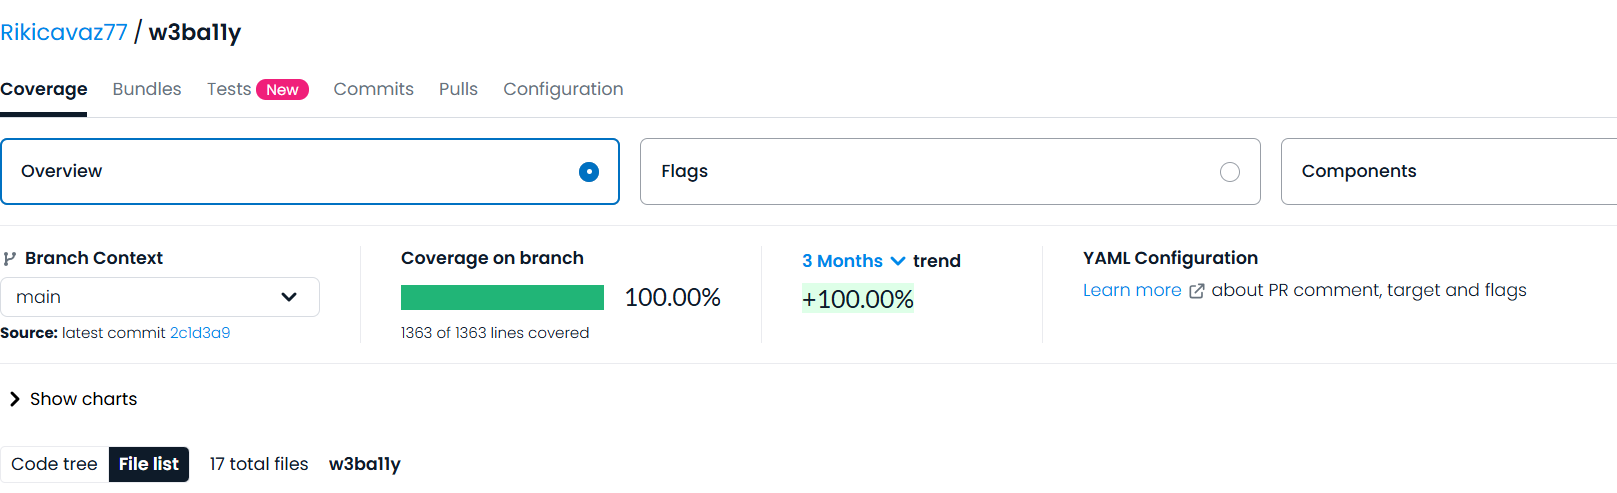
\includegraphics[width=0.9\columnwidth]{test/coverage.png}}
  \caption{Copertura del codice - report di Codecov}
\end{figure}

\par\noindent I test automatici vengono eseguiti a ogni apertura, aggiornamento o chiusura di una pull request, garantendo che tutto il codice rilasciato superi i test e mantenga una copertura uniforme. Dal punto di vista architetturale e organizzativo, i test rispecchiano fedelmente la struttura del core dell’estensione, risultando più leggibili e manutenibili. 

\vspace{10pt}
\begin{samepage}
  \dirtree{%
    .1 tests.
    .2 controller.
    .2 model.
    .2 services.
    .3 strategy.
    .2 utils.
    .2 view.
  }
\end{samepage}

\vspace{10pt}
\par\noindent Per mantenere l’isolamento tra l’ambiente di test e il resto dell’applicazione, ciascun file testato deve terminare con la seguente porzione di codice:

\vspace{10pt}
\begin{samepage}
\begin{lstlisting}[language=JavaScript]
  /* istanbul ignore next */
  if (typeof module !== 'undefined' && typeof module.exports !== 'undefined') {
    module.exports = KeywordHighlighter;
  }
\end{lstlisting}
\end{samepage}

\vspace{10pt}
\par\noindent Questo approccio consente di importare i moduli all’interno dei file di test tramite la seguente istruzione:

\vspace{10pt}
\begin{samepage}
\begin{lstlisting}[language=JavaScript]
  const KeywordHighlighter = require('@keyword/services/keyword_highlighter');
\end{lstlisting}
\end{samepage}

\vspace{10pt}
\par\noindent Di seguito sono riportati i test di unità e di integrazione.